\section{Design of PCStream}
In this section, we describe in detail the proposed automatic stream management
technique, {\sf PCStream}.  We first explain a mechanism that automatically
obtains PC values at runtime, and then describe how multiple data with
different PC values are combined and delivered to an SSD. Finally, we introduce
a two-phase data separation technique that further optimizes {\sf PCStream}.

\begin{figure}[b]
	\centering
	\vspace{-15pt}
	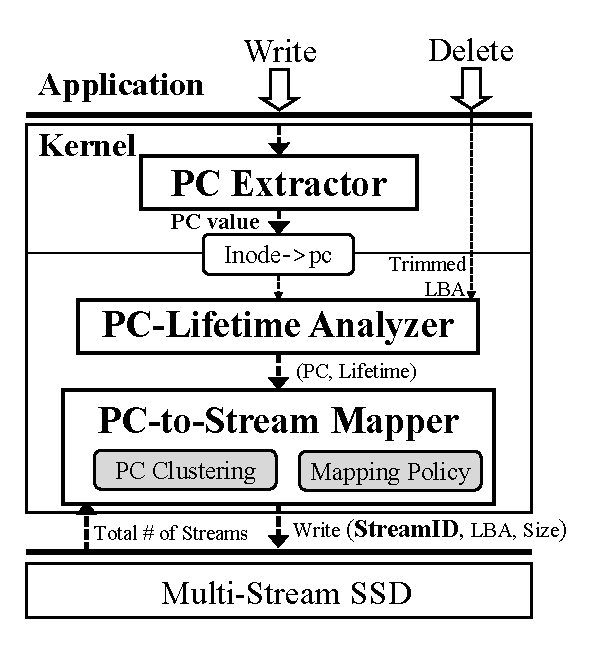
\includegraphics[width=0.6\linewidth]{figure/architecture4}
	\vspace{-10pt}
	\caption{An overall architecture of {\sf PCStream}}
	\label{fig:architecture}
\end{figure}

Fig.~\ref{fig:architecture} shows the overall architecture of {\sf PCStream},
which is composed of a \textit{PC extractor}, a \textit{PC lifetime analyzer},
and a \textit{PC-to-stream mapper}.  The PC extractor is implemented in the
Linux kernel as part of a system call handler. Its responsibility is for
intercepting write-related system calls (e.g., \texttt{write()}) and extracting
a PC value.  This enables us to keep track of PCs corresponding to new data
written by a specific module of an application.  The obtained PC is stored in
an inode data structure of a file system (modified for \textsf{PCStream}) and
is delivered to the lifetime analyzer implemented in a block layer.  The
lifetime analyzer estimates expected lifetimes of data belonging to a given PC.
To know when data is deleted, the lifetime analyzer also intercepts TRIM
requests from a file system.  Based on the lifetime information, the
PC-to-stream mapper clusters PC values with similar lifetimes and maps them
together to the same stream ID.  This mapping is required because of the
limited number of streams supported by an SSD.

\vspace{-5pt}
\subsection{Automatic PC computation}
As mentioned earlier, a PC is defined as the sum of program counters along the
execution path of a function call that finally reaches a \texttt{write()}
system call.  A function call involves pushing the next program counter to the
stack as a return address, which is used as a return location to keep
executing a caller when a callee function is finished.  In general, by
using a frame register, we are able to back-track the stack frames of the
process and selectively get return addresses, which are then used for
computing a PC value. For example, Fig.~\ref{fig:getpc}(a) illustrates how a PC
value is obtained by back-tracking the stack.

Unfortunately, C/C++ compilers often optimize an output code so
that it does not use a frame register if possible.  One example is a
{\tt -fomit-frame-pointer} option of GCC. While it is effective in saving
precious resources like CPU registers, this makes it difficult for us to
back-track return addresses only. One alternative is fully examine
every word in the stack and find out ones that point to the code
segment of the process's virtual address.  Modern OSes divide the process's
virtual address into segments for their purposes, and thus program instructions
(code) are stored in a specific range of the virtual address space (e.g.,
{\texttt{0x400000h}} to {\texttt{0x40c000h}} in the
Linux).  If there are words that hold a value pointing to somewhere in the code
segment, they are highly likely to be one of the return values.  
\begin{comment} % DO NO REMOVE
Moreover, since the PC extractor is implemented in the kernel, it is not only
able to access the entire virtual address of a process, but also know the
address space layout.
\end{comment}

Searching the entire process stack would require long CPU time. Thus, the
search process stops when a sufficient number of return addresses are found in
the stack. Currently, this threshold value is set to 5.  In our experiments
with a 3.4 GHz CPU machine, the search process only takes 300-400 $n$sec per
write system call, on average, so its overhead is not so huge.
Fig.~\ref{fig:getpc}(b) illustrates how PC computation works in {\sf PCStream}
in detail.

\begin{figure}[t]
	\centering
	\subfloat[with frame pointer]{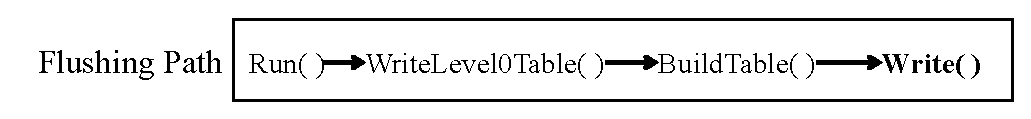
\includegraphics[width=0.21\textwidth]{figure/getpc_1}}  
	%\hspace{10pt}
	\subfloat[without frame pointer]{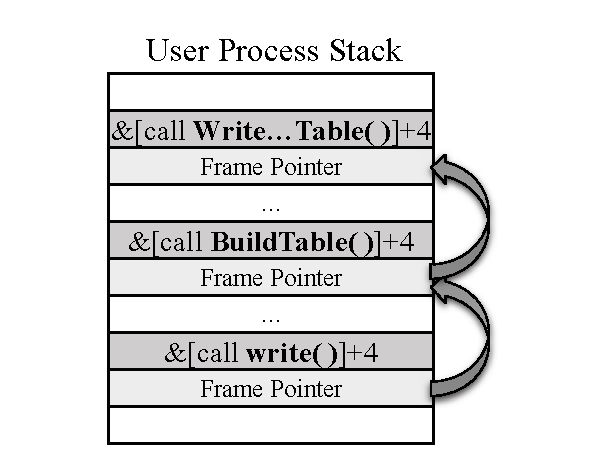
\includegraphics[width=0.23\textwidth]{figure/getpc_2}}
	\vspace{-10pt}
	\caption{PC extractions with or without the frame pointer.}
	\label{fig:getpc}
	\vspace{-15pt}
\end{figure}


\vspace{-5pt}
\subsection{PC lifetime prediction}
The prediction of PC lifetimes is rather complicated. The lifetime of
append-only data is defined as from when they are appended to the storage to
when they are deleted by an application. The time at which data belonging to a
certain PC is written can be obtained through the PC extractor. To know when
the data is removed, however, we should be able to monitor TRIM commands from a
file system that invalidate previously written data.  To keep track of the
lifetimes of data written by a specific PC, the lifetime analyzer maintains a
list of LBAs for PCs when the LBAs are being written.  Upon receiving TRIM
commands destined for those LBAs, the lifetime analyzer is able to measure the
exact lifetime of those data. In append-only applications, a large chunk of
data are written and invalidated together (e.g., 64 MB in RocksDB), and thus
LBAs belonging to the same PC tend to have the similar lifetime. Note that, the
same PC generates multiple data streams with different lifetimes, so the
average of them is used as PC's expected lifetime.


\vspace{-5pt}
\subsection{Mapping PCs to SSD stream}
Our next step is to map a group of PCs with similar lifetimes to an SSD stream.
This is because of a limited number of stream IDs offered by an SSD. For
example, SSDs used in FStream~\cite{FStream} and AutoStream~\cite{AutoStream}
support only 9 and 16 streams, respectively. To properly group multiple PCs,
the PC-to-stream mapper employs a simple 1-D clustering algorithm, which is a
sort of like the Jenks optimization method~\cite{Jenks}.  For all the PCs, the
mapper internally builds a 1-D array sorted by PCs' lifetimes.  Given an
available SSD stream number, it runs the clustering algorithm and determines
the best arrangement of PCs into different classes.  To adapt to changing
workloads, reclustering operations should be regularly performed. Since the
number of PCs created by applications is not limited, the clustering algorithm
must be efficient enough to quickly handle many PCs. Our goal in this work is
to confirm the feasibility of using the PC for multi-streamed SSDs, so we leave
those issues as our future work.


\vspace{-5pt}
\subsection{\textcolor{red}{Two-phase stream assignment}}
\begin{figure}[!t]
\centering
\hspace{1pt}
\subfloat[compaction: all levels]{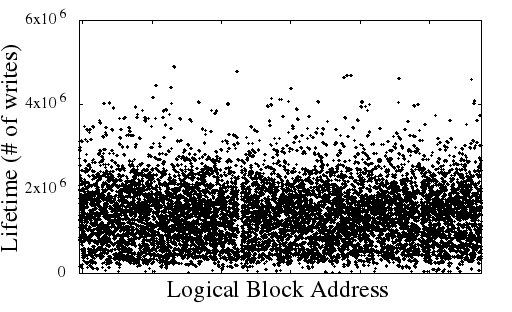
\includegraphics[width=0.23\textwidth]{figure/pc_3b}}
\subfloat[compaction: L2]{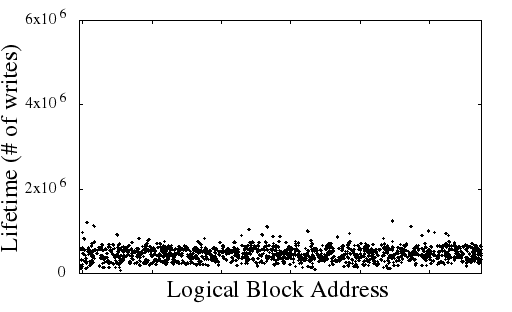
\includegraphics[width=0.23\textwidth]{figure/type_4b}}  % data from 4/03040047
\hfill
\vspace{-10pt}
\subfloat[compaction: L3]{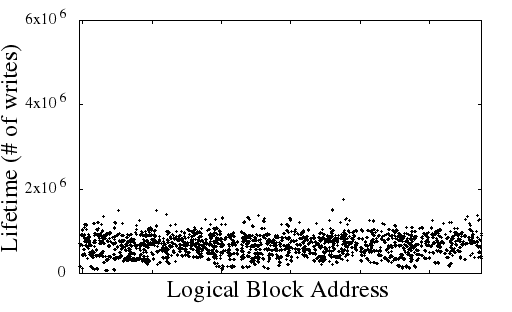
\includegraphics[width=0.23\textwidth]{figure/type_5b}}
\subfloat[compaction: L4] {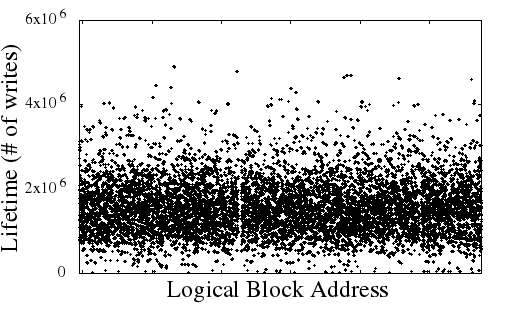
\includegraphics[width=0.23\textwidth]{figure/type_6b}}
\vspace{-10pt}
\caption{The lifetime distribution of compaction context.} 
\label{fig:compaction}
\vspace{-15pt}
\end{figure}

While the PC can be used as a useful indicator that determines the lifetime of
data, we also observe that the same PC could generate data with various
lifetimes. One example is the compaction module of RocksDB. RocksDB maintains
several levels, L1, ..., L$n$, in the persistent storage, except for L0 (or a
memtable) stored in DRAM.  Once one level, say L2, becomes full, all the data
in L2 is compacted to a lower level, i.e., L3.  It involves moving data from L2
to L3, along with the deletion of the old data in L2.  In the
LSM-tree~\cite{LSM}, a higher level is smaller than a lower level (i.e., L2 $<$
L3). Thus, data stored in a higher level is invalidated sooner than those kept
in lower levels, thereby having shorter lifetimes.

%Once the L1 becomes full,
%\textit{all} the data kept in the L1 are moved to the L2 by the compaction
%module.  The same operation is applied to the other levels (i.e., L3, ...,
%L$n-1$).  The compaction involves reading and writing data from a higher level
%(e.g., L1) to a lower level (e.g., L2).  The data in a higher level (e.g., L1)
%is then removed.  

%While the program context can be used as a useful indicator that determines the
%lifetime of data, we also observe that the same PC could generate data 
%with diverged lifetimes. One of the representative examples is the compaction
%module of RocksDB. RocksDB maintains several levels, L1, ..., L$n$, in the
%persistent storage, except for L0 (or a memtable) stored in DRAM.  Data flushed
%from the memtable are first written to the L1.  Once the L1 becomes full,
%\textit{all} the data kept in the L1 are moved to the L2 by the compaction
%module.  The same operation is applied to the other levels (i.e., L3, ...,
%L$n-1$).  The compaction involves reading and writing data from a higher level
%(e.g., L1) to a lower level (e.g., L2).  The data in a higher level (e.g., L1)
%is then removed.  In the LSM-tree, a higher level is smaller than a lower
%level. Thus, data stored in a higher level is invalidated sooner than data kept
%in lower levels, thereby having much shorter lifetimes.

Unfortunately, the compaction is done by the same module for all the levels.
PC is thus not useful to distinguish data written for different levels.
Fig.~\ref{fig:compaction}(a) shows the lifetimes of data written by the
compaction module.  Figs.~\ref{fig:compaction}(b)-(d) illustrate the lifetimes
of data when different PC numbers are assigned to each level by modifying the
code.  Data from L1 are likely to have shorter lifetime, while L4 has generally
long-lived data.

In order to automatically assign data from the same PC to different SSD streams
according to their lifetimes, we propose a two-phase method that decides SSD
stream IDs in both a host and an SSD level.  {\sf PCStream} roughly assigns a
stream ID based on a PC value.  An FTL running inside an SSD uses this stream
ID as a guideline and prevents data with different stream IDs from being mixed
up in the same flash blocks. The FTL then decides a substream ID during garbage
collection (GC). If there are valid data in a victim block for GC, it means
that those data tend to have longer lifetimes compared to other data even if
they belong to the same stream. Thus, the FTL splits the SSD stream into two
substreams.  The first is for relatively hot data that were invalidated
earlier; the second is for relatively cold ones that are still valid in the
victim.  After that, data with different substream IDs are isolated in
different blocks. 

